\documentclass[twoside,11pt,nolof]{starlink}

% -----------------------------------------------------------------------------
\stardoccategory    {Starlink User Note}
\stardocinitials    {SUN}
\stardocsource      {sun\stardocnumber}
\stardoccopyright   {Copyright \copyright\ 2014 University of%
 British Columbia and the Science \& Technology Facilities Council}
\stardocnumber      {264.0}
\stardocauthors     {Andrew G. Gibb \& Tim Jenness}
\stardocdate        {10 Jun 2014}
\stardoctitle       {ORAC-DR --- SCUBA-2 Pipeline Data Reduction}
\stardocversion     {Version 1.4.0}
\stardocmanual      {User's Guide}
\stardocabstract  {
  The \oracdr\ data reduction pipeline is designed to reduce data from
  many different instruments. This document describes how to use
  \oracdr\ to process data taken with the SCUBA-2 instrument on the
  James Clerk Maxwell Telescope.
}

% -----------------------------------------------------------------------------

% +
%  Name:
%     sun264.tex
%
%  Purpose:
%     Documentation for SCUBA-2 data reduction with ORAC-DR
%
%  Authors:
%     AGG: Andy Gibb (UBC)
%
%  History:
%     2010-10-26 (AGG):
%        Initial version
%     2012-07-25 (AGG):
%        Updates for Kapuahi
%     2013-03-01 (AGG):
%        Updates for Hikianalia
%     {Add further history here}
%
% -

\stardocname  {\stardocinitials /\stardocnumber}

% Document specific \providecommand or \newenvironment commands.

% A new environment for quoting verbatim
% Environment for indenting and using a small font.
\newenvironment{myquote}{\begin{quote}\begin{small}}{\end{small}\end{quote}}

\providecommand{\starlink}{\htmladdnormallink{Starlink}{http://starlink.eao.hawaii.edu}}

% Shorthand and HTML references for other Starlink tasks
\providecommand{\CCDPACK}{\textsc{ccdpack}}
\providecommand{\CCDPACKref}{\xref{\CCDPACK}{sun139}{}}
\providecommand{\CUPID}{\textsc{cupid}}
\providecommand{\CUPIDref}{\xref{\CUPID}{sun255}{}}
\providecommand{\CURSA}{\xref{\textsc{cursa}}{sun190}{}}
\providecommand{\FIGARO}{\textsc{figaro}}
\providecommand{\FIGAROref}{\xref{\FIGARO}{sun86}{}}
\providecommand{\FLUXES}{\textsc{fluxes}}
\providecommand{\FLUXESref}{\xref{\FLUXES}{sun213}{}}
\providecommand{\GAIA}{\textsc{gaia}}
\providecommand{\GAIAref}{\xref{\GAIA}{sun214}{}}
\providecommand{\HDSTRACE}{\textsc{hdstrace}}
\providecommand{\HDSTRACEref}{\xref{\HDSTRACE}{sun102}{}}
\providecommand{\KAPPA}{\textsc{kappa}}
\providecommand{\KAPPAref}{\xref{(SUN/95)}{sun95}{}}
\providecommand{\PHOTOM}{\textsc{photom}}
\providecommand{\PHOTref}{\xref{(SUN/45)}{sun45}{}}
\providecommand{\SMURF}{\textsc{smurf}}
\providecommand{\SMURFcooksro}{\xref{SC/19}{sc19}{}}
\providecommand{\SMURFcook}{\xref{SC/21}{sc21}{}}
\providecommand{\SMURFsun}{\xref{SUN/258}{sun258}{}}
\providecommand{\ADAMsgref}{\xref{SG/4}{sg4}{}}
\providecommand{\ADAMsunref}{\xref{SUN/101}{sun101}{}}
\providecommand{\astref}{\xref{SUN/211}{sun211}{}}
\providecommand{\ndfref}{\xref{SUN/33}{sun33}{}}

\providecommand{\oracdr}{\textsc{orac-dr}}
\providecommand{\oracsun}{\xref{SUN/230}{sun230}{}}
\providecommand{\scubasun}{\xref{SUN/231}{sun231}{}}
\providecommand{\picard}{\textsc{picard}}
\providecommand{\picardsun}{\xref{SUN/265}{sun265}{}}

% Application tasks
\providecommand{\task}[1]{\textsf{#1}}

% SMURF tasks
\providecommand{\badbolos}{\xref{\task{badbolos}}{sun258}{BADBOLOS}}
\providecommand{\calcdark}{\xref{\task{calcdark}}{sun258}{CALCDARK}}
\providecommand{\calcflat}{\xref{\task{calcflat}}{sun258}{CALCFLAT}}
\providecommand{\calcnoise}{\xref{\task{calcnoise}}{sun258}{CALCNOISE}}
\providecommand{\calcresp}{\xref{\task{calcresp}}{sun258}{CALCRESP}}
\providecommand{\copyflat}{\xref{\task{copyflat}}{sun258}{COPYFLAT}}
\providecommand{\dreamsolve}{\xref{\task{dreamsolve}}{sun258}{DREAMSOLVE}}
\providecommand{\dreamweights}{\xref{\task{dreamweights}}{sun258}{DREAMWEIGHTS}}
\providecommand{\gsdtoacsis}{\xref{\task{gsd2acsis}}{sun258}{GSD2ACSIS}}
\providecommand{\gsdshow}{\xref{\task{gsdshow}}{sun258}{GSDSHOW}}
\providecommand{\smurfhelp}{\xref{\task{smurfhelp}}{sun258}{SMURFHELP}}
\providecommand{\impaztec}{\xref{\task{impaztec}}{sun258}{IMPAZTEC}}
\providecommand{\makecube}{\xref{\task{makecube}}{sun258}{MAKECUBE}}
\providecommand{\qlmakemap}{\xref{\task{qlmakemap}}{sun258}{QLMAKEMAP}}
\providecommand{\rawunpress}{\xref{\task{rawunpress}}{sun258}{RAWUNPRESS}}
\providecommand{\rawfixmeta}{\xref{\task{rawfixmeta}}{sun258}{RAWFIXMETA}}
\providecommand{\sctwosim}{\xref{\task{sc2sim}}{sun258}{SC2SIM}}
\providecommand{\sctwothreadtest}{\xref{\task{sc2threadtest}}{sun258}{SC2THREADTEST}}
\providecommand{\scanfit}{\xref{\task{scanfit}}{sun258}{SCANFIT}}
\providecommand{\skynoise}{\xref{\task{skynoise}}{sun258}{SKYNOISE}}
\providecommand{\smurfcopy}{\xref{\task{smurfcopy}}{sun258}{SMURFCOPY}}
\providecommand{\stackframes}{\xref{\task{stackframes}}{sun258}{STACKFRAMES}}
\providecommand{\starecalc}{\xref{\task{starecalc}}{sun258}{STARECALC}}
\providecommand{\timesort}{\xref{\task{timesort}}{sun258}{TIMESORT}}
\providecommand{\unmakecube}{\xref{\task{unmakecube}}{sun258}{UNMAKECUBE}}

\providecommand{\extinction}{\xref{\task{extinction}}{sun258}{EXTINCTION}}
\providecommand{\flatfield}{\xref{\task{flatfield}}{sun258}{FLATFIELD}}
\providecommand{\jcmtstate}{\xref{\task{jcmtstate2cat}}{sun258}{JCMTSTATE2CAT}}
\providecommand{\dumpocscfg}{\xref{\task{dumpocscfg}}{sun258}{DUMPOCSCFG}}
\providecommand{\makemap}{\xref{\task{makemap}}{sun258}{MAKEMAP}}
\providecommand{\gettsys}{\xref{\task{gettsys}}{sun258}{GETTSYS}}

\providecommand{\remsky}{\xref{\task{remsky}}{sun258}{REMSKY}}
\providecommand{\clean}{\xref{\task{sc2clean}}{sun258}{SC2CLEAN}}
\providecommand{\concat}{\xref{\task{sc2concat}}{sun258}{SC2CONCAT}}
\providecommand{\fft}{\xref{\task{sc2fft}}{sun258}{SC2FFT}}
\providecommand{\fts}{\xref{\task{sc2fts}}{sun258}{SC2FTS}}

\providecommand{\rebin}{\texttt{rebin}}
\providecommand{\iterate}{\texttt{iterate}}

% Other tasks
\providecommand{\autophotom}{\xref{\task{autophotom}}{sun45}{AUTOPHOTOM}}
\providecommand{\beamfit}{\xref{\task{beamfit}}{sun95}{BEAMFIT}}
\providecommand{\csub}{\xref{\task{csub}}{sun95}{CSUB}}
\providecommand{\clinplot}{\xref{\task{clinplot}}{sun95}{CLINPLOT}}
\providecommand{\collapse}{\xref{\task{collapse}}{sun95}{COLLAPSE}}
\providecommand{\display}{\xref{\task{display}}{sun95}{DISPLAY}}
\providecommand{\fitsedit}{\xref{\task{fitsedit}}{sun95}{FITSEDIT}}
\providecommand{\fitslist}{\xref{\task{fitslist}}{sun95}{FITSLIST}}
\providecommand{\kapdiv}{\xref{\task{div}}{sun95}{DIV}}
\providecommand{\mlinplot}{\xref{\task{mlinplot}}{sun95}{MLINPLOT}}
\providecommand{\ndfcopy}{\xref{\task{ndfcopy}}{sun95}{NDFCOPY}}
\providecommand{\provshow}{\xref{\task{provshow}}{sun95}{PROVSHOW}}
\providecommand{\thresh}{\xref{\task{thresh}}{sun95}{THRESH}}
\providecommand{\wcsalign}{\xref{\task{wcsalign}}{sun95}{WCSALIGN}}
\providecommand{\wcsattrib}{\xref{\task{wcsattrib}}{sun95}{WCSATTRIB}}
\providecommand{\wcsmosaic}{\xref{\task{wcsmosaic}}{sun95}{WCSMOSAIC}}
\providecommand{\makemos}{\xref{\task{makemos}}{sun139}{MAKEMOS}}
\providecommand{\topcat}{\xref{\textsc{Topcat}}{sun253}{}}

% Constants
\providecommand{\snrmin}{100}

% macros for typesetting parameters
\providecommand{\aparam}[1]{\texttt{#1}}     % ADAM parameter
\providecommand{\cparam}[1]{\texttt{#1}}     % CONFIG parameter
\providecommand{\ndfcomp}[1]{\texttt{#1}}    % NDF component


% -----------------------------------------------------------------------------
\begin{document}
\scfrontmatter

\newpage
\section{\xlabel{introduction}Introduction\label{se:intro}}

The SCUBA-2 pipeline is a suite of recipes and primitives for the
\oracdr\ automated data processing software package. Additional
functionality for processing and analysis of reduced data is provided
through a number of \picard\ recipes. General documentation on
\oracdr\ and \picard\ can be found in \oracsun\ and
\picardsun\ respectively.

The fundamental operation of the pipeline is to begin with raw data
and produce calibrated science images with no additional user
input. All decisions are based on metadata stored in the data files
combined with basic quality assessment of reduced data products.

\subsection{Document conventions}

In an attempt to make this document clearer to read, different fonts
are used for specific structures.

Observing modes are denoted by all upper case body text (e.g.\
FLATFIELD).

Starlink package names are shown in small caps (e.g.\ \SMURF);
individual task names are shown in sans-serif
(e.g.\ \makemap). \oracdr\ recipes and primitives are also shown in
sans-serif and are always upper case (e.g.\ \task{REDUCE\_SCAN}).

Content listings are shown in fixed-width type (sometimes called
`typewriter'). Extensions and components within NDF (\ndfref) data
files are shown in upper case fixed-width type (e.g.\
\ndfcomp{HISTORY}).

Text relating to filenames (including suffices for data products), key
presses or entries typed at the command line are also denoted by
fixed-width type (e.g.\ \texttt{\% smurf}), as are parameters for
tasks which are displayed in upper case (e.g.\ \aparam{METHOD}).

References to Starlink documents, i.e., Starlink User Notes (SUN),
Starlink General documents (SG) and Starlink Cookbooks (SC), are given
in the text using the document type and the corresponding number
(e.g.\ SUN/95). Non-Starlink documents are cited in the text and
listed in the bibliography.

File name suffices represent the text between the final underscore
character and the three-letter \verb+.sdf+ extension. For example, a
file named \verb+s4a20101020_00002_0001_cal.sdf+ has the suffix
\verb+_cal+.

\newpage
\section{\xlabel{pipelines}SCUBA-2 Pipeline Variants\label{se:pipelines}}

There are three variants of the SCUBA-2 pipeline, users will likly only need
to run the science pipeline. The other two pipelines are designed to run in
real time at the JCMT. 

\begin{itemize}
\item The science pipeline has access to all the data observed for a
  given project and adopts a best-possible reduction approach. Images
  are made for each complete observation which are combined to create
  the final image.

\item The quick-look (QL) pipeline is primarily designed to perform
  quality-assurance analysis of the incoming data for real-time
  assessment of the instrument performance. It is also responsible for
  processing pointing and focus data.

\item The summit pipeline runs in parallel with the QL pipeline
  (though on a different machine) and is the primary image-processing
  pipeline. Processing is delayed until sufficient data exist to
  produce a higher quality image. In practice this happens after a
  certain time has elapsed since an image was last made.
\end{itemize}

\subsection{Requirements for running the SCUBA-2 pipeline}

The SCUBA-2 pipeline requires a recent Starlink installation. The
latest version may be obtained from
\htmladdnormallink{\texttt{http://starlink.eao.hawaii.edu/starlink}}{http://starlink.eao.hawaii.edu/starlink}. Since
development of the pipeline is an ongoing process, it is recommended
that the newest builds be used to access the full capabilities of the
pipeline. These builds can be obtained from\\
\htmladdnormallink{\texttt{http://starlink.eao.hawaii.edu/starlink/rsyncStarlink}}{http://starlink.eao.hawaii.edu/starlink/rsyncStarlink}
and may be kept up-to-date with rsync.

The Starlink Perl installation (Starperl) must be used to run the
pipeline due to the module requirements. The Starlink environment should be
initialized as usual before running \oracdr.

The software used to process raw data into images is called the
SubMillimetre User Reduction Facility (\SMURF). Detailed documentation
on \SMURF\ can be found in \SMURFsun, while \SMURFcook\ is a cookbook
that describes some of the background to SCUBA-2 data reduction.

The pipeline uses the following Starlink applications:
\begin{itemize}
\item \SMURF
\item \KAPPA
\item \FLUXES
\item \FIGARO
\item \CCDPACK
\item \CUPID
\end{itemize}

\subsection{Important environment variables}

The pipeline uses a number of environment variables to determine where
data should be read from and written to. Some are set automatically
when the pipeline is initialized, but they can be overridden manually
and, with the \verb+-honour+ flag may be left unchanged between
successive runs of the pipeline. The variables that must be defined in
order for the pipeline to run are denoted as `Mandatory' in the list
below.

\begin{itemize}

\item \verb+STARLINK_DIR+: location of the user's Starlink
  installation. [Mandatory]

\item \verb+ORAC_DATA_IN+: the location where data are read from. If
  running with \verb+-loop flag+, this is the location of the flag
  files, rather than the data files. [Mandatory]

\item \verb+ORAC_DATA_OUT+: location where pipeline data products are
  written. Also used as a location for user-specified configuration
  files for \task{makemap}. [Mandatory]

\item \verb+ORAC_DATA_ROOT+: root location for data. At the JCMT,
  this is \verb+/jcmtdata/raw/scuba2+. If not defined, the current
  directory is assumed. [Optional]

\item \verb+MAKEMAP_CONFIG_DIR+: a user-specified location for
  \task{makemap} configuration files. [Optional]

\item \verb+FINDCLUMPS_CONFIG_DIR+: a user-specified location for
  \task{findclumps} configuration files. [Optional]

\end{itemize}


As an example, to set up or override the pipeline environment variables, tcsh users will need to do:

\begin{terminalv}
% setenv ORAC_DATA_IN folder1/
% setenv ORAC_DATA_OUT folder2/
\end{terminalv}

and bash users will need to do:

\begin{terminalv}
$ export ORAC_DATA_IN=folder1/
$ export ORAC_DATA_OUT=folder2/
\end{terminalv}
 

\subsection{Getting help}

Basic help and a list of command-line options may be obtained after
initializing \oracdr\ by running :
\begin{terminalv}
% oracdr -h
\end{terminalv}
or
\begin{terminalv}
% oracdr -man
\end{terminalv}

More complete documentation on \oracdr\ can be found in \oracsun.


\newpage
\section{\xlabel{overview}Overview of the SCUBA-2 pipeline\label{se:overview}}

\subsection{Science pipeline}

The science pipeline examines all the data files given to it and works
out which files are related and should be processed together
(``batch'' mode). Each observation is still processed separately to
produce an image, which is calibrated in mJy\,beam$^{-1}$ (unless
otherwise specified by the recipe). All the images for a given source
are combined into a single coadd using inverse-variance weighting. If
the source is a known calibrator then the images are checked for
offsets and, if necessary, shifted to place the source at the correct
position.

At the end of processing, all temporary files are deleted: the only
data files left on disk will have the suffix \verb+_reduced+.

Recipes exist for a number of different target types which contain
different processing steps, relevant to each particular target
type. These are bright or faint compact (such as planets, T-Tauri
stars or extragalactic blank fields respectively) and extended (such
as Galactic star-forming regions). Examples of these steps include
applying a matched-filter to enhance point-source detectability or
running a clump-finding algorithm.

Note that additional recipes exist for determining the noise
properties of the science data. The first performs the same noise
analysis and QA checks as the QL pipeline. This can be run offline by
adding the recipe name ASSESS\_DATA\_NOISE to the \oracdr\ command
line. The second recipe calculates the noise and NEP properties in
addition to carrying out the standard map-making procedure, and
compares the noise properties with that expected from the SCUBA-2
integration time calculator. This recipe is called
REDUCE\_SCAN\_CHECKRMS. See the documentation below for further
details.

\subsection{Quicklook (QL) pipeline}

The QL pipeline uses a task called \verb+qlgather+ to monitor the
DRAMA processes and write out a flag file with the names of the files
to process. The pipeline reads that flag file and processes each of
the named files. \verb+qlgather+ collates data with the same subscan
number. If new data are detected before all the expected files for
the current subscan are in place, the new data take precedence and
processing of the current subscan may be skipped.

Fastramp flatfields taken as part of each observation are processed
and stored in the calibration system. The responsivity image for all
four subarrays (along with the previous and percentage-change images)
are displayed in a Kapview window.

Pointing and focus data are processed using the iterative map maker
with a configuration file optimized for such observations of bright
compact sources. Corresponding fastramp flatfields are obtained from
the calibration system. For pointing observations an FCF is derived if
the source is a known calibrator. The image is displayed using \GAIA,
showing in window 1, and then combined with the current coadd image
(if one exists). The coadd image is displayed in another \GAIA\ window
(2), and its error component (noise) in another (3). For focus
observations, the data for each SMU position is processed separately
and combined into a three-dimensional data cube. The name of the
pointing coadd or focus cube is written to a flag file
(\verb+.sYYYYMMDD_MMMMM.ok+, where \verb+MMMMM+ is the current
observation number) for further analysis by the telescope
POINTING\_FOCUS task. The pipeline makes its own estimates of the
pointing and focus solution, which are written to log files. Any
temporary files created during this processing are deleted, keeping
only files with a suffix \verb+_reduced+ or \verb+_foc+ for pointing
and focus respectively.

Science data are processed as noise observations. The noise between 2
and 10 Hz is calculated along with the noise equivalent power (NEP)
and the weighted NEP. These values undergo quality assurance checks to
ascertain whether or not the instrument is still operating within
specified limits. The focal-plane noise distribution is displayed in a
Kapview window.

Data from other observing modes are processed as per their own recipes.

\subsection{Summit pipeline}

The summit pipeline is the main image-making pipeline running at the
telescope. It will use all available data for processing (unlike the
QL which will skip data to deal with the latest files), and as such
may fall behind for several subscans. However, the processing is
structured such that the processing for a given observation should be
complete before a new observation begins.

Pointing and focus observations (along with setups, noise and skydips)
are processed in a similar manner to the QL, though no data are
skipped.

The pipeline checks for the presence of flag files which are updated
with the names of new data as they are written to disk. As each file
is picked up by the pipeline, it checks to see how much time has
elapsed since the last map was made. If the time exceeds a threshold
(typically about one-and-a-half to two minutes), then a new map is
made using all of the data taken since the previous map. The map is
calibrated in mJy\,beam$^{-1}$ using the standard FCF. If it is too
soon to make a new map, the raw data are flatfielded and left on disk
(suffix \verb+_ff+). These files will be deleted once a new image is
made.

The new image is combined with the existing coadd (if appropriate) and
a new NEFD image is calculated. Note that the summit pipeline coadds
images for a given source across multiple observations so fainter
features will be revealed as the integration time increases. If a new
image was not created during the latest pass through the recipe then
all flatfielded data files needed to create a map are left on disk.



\newpage
\section{\xlabel{offline}Science pipeline processing of SCUBA-2 data\label{se:offline}}

\subsection{Running the science pipeline at your home institution}

If the data for your project have been downloaded from CADC and placed
in a single directory, the easiest procedure is to create a text file
containing the name of each of these raw files. That file should
contain either the full path to each file or relative to the current
directory (or the directory defined by \verb+ORAC_DATA_IN+). The data
can be processed with the commands:
\begin{terminalv}
% oracdr_scuba2_XXX -cwd
% oracdr -loop file -files <list_of_files>
\end{terminalv}
where \verb+XXX+ is the wavelength (450 or 850). An optional UT
observation date in the form \verb+YYYYMMDD+ may be given
(e.g.\ 20100301). If the date is omitted, the current date is assumed
- however, the file naming convention uses the date on which the data
were taken. The initialization command only needs to be run once per
UT date, and may be given the \verb+-honour+ flag to use existing
definitions of the relevant environment variables. Alternatively, the
\verb+-cwd+ flag may be given to force the pipeline to use the current
working directory for all input and output.

Note that there is no need to uncompress the data files prior to
running the pipeline: \oracdr\ can accept files compressed with
\verb+gzip+ (ending \verb+.sdf.gz+) and will uncompress them
itself. However, be aware that the uncompressed files are not deleted
at the end of processing (\oracdr\ does not delete raw data).

Each observation is processed separately and the images combined to
form a single output image. If the list of files contains data from
multiple sources, the pipeline will treat each source separately and
create different output files accordingly. Calibration is handled
automatically (see \ref{sse:cal} below).

The default science recipes will display the individual observation
images plus the final coadded image using \GAIA. (The display can be
turned off, if desired, by adding \texttt{-nodisplay} to the
\oracdr\ command line.)

\subsection{Pipeline products}

The science data products from the pipeline have a suffix of
\verb+_reduced+. The files beginning with \verb+s+ are the products
from individual observations; the files beginning \verb+gs+ are the
coadded observations for a single object. The products from
non-science observations may have different suffices, and may be
three-dimensional cubes. See the documentation on the individual
recipes in Appendix\,\ref{ap:classified} for further details on those
products.

In addition to the data files, the reduced products have PNG format
images 64, 256 and 1024 pixels on a side for easy viewing in an image
viewer or web browser.

\subsection{Calibration\label{sse:cal}}

If no calibration observations are available, and unless otherwise
instructed, the pipeline will apply standard flux conversion factors
(FCFs) to calibrate the images in mJy\,beam$^{-1}$. Currently these
are 537000 mJy\,beam$^{-1}$ at 850\,$\mu$m and 491000 at
450\,$\mu$m. (See also \cite{scuba2calpaper}.)

\subsection{Customizing the map-making}

The pipeline uses the \SMURF\ dynamic iterative map-maker (\makemap)
to create maps from raw data. A detailed description of the map-maker
is given in \SMURFcook\ and \cite{smurfpaper}. The map-maker uses a
configuration file to control the data processing which may be
modified by users with advanced knowledge of the map maker. The
SCUBA-2 pipeline may be given the name of an alternative or customized
configuration file via the recipe parameter capability of \oracdr. A
number of pre-defined configuration files exist in the directory
\verb+$STARLINK_DIR/share/smurf+.

Once a suitable configuration file has been created, add its name to a
recipe parameter file as follows:
\begin{terminalv}
[REDUCE_SCAN]
MAKEMAP_CONFIG = myconfigfilename.lis
\end{terminalv}
and add \texttt{-recpars recipe\_params.lis} to the command line when
running the pipeline, where \verb+recipe_params.lis+ is the name of
recipe parameter file (which must be in the current directory if the
path is not given). The \task{makemap} configuration file must exist
in the current working directory or one of the directories defined by
the environment variables \verb+MAKEMAP_CONFIG_DIR+,
\verb+ORAC_DATA_OUT+, or \verb+ORAC_DATA_CAL+ or in
\verb+$STARLINK_DIR/share/smurf+. Each directory is searched in this
order and the first match is used.

Note that if running a recipe other than REDUCE\_SCAN (such as one of
the dedicated JLS recipes) that recipe name should be placed in square
brackets instead.

\subsection{Running the science pipeline at EAO/JCMT}

The raw data are stored at EAO in the same way as at the summit. (It
is also possible to do this yourself at your home institution but in
general will not be worth the effort: use the example above instead.)
The machine \verb+sc2dr5+ is available at the summit for general user
data processing.

If processing data from a single night, then \oracdr\ can be run with
the \texttt{-loop flag} option to indicate that the pipeline should
examine the contents of flag files (which end in \verb+.ok+). The flag
files contain the path to the files to be processed, and have a fixed
naming convention so the pipeline can recognize them. Use the
\texttt{-list} option to specify the observation numbers to be
processed (otherwise the pipeline will begin at observation 1). The
command \verb+scuba2_index+ will produce a summary of the available
data.

If processing data from multiple nights, create a text file with the
names of the relevant data files, as for running at your home
institution above, and follow the same procedure.

\subsection{Processing examples\label{sse:examples}}

To process a set of data downloaded from the JCMT archive at CADC,
where the files to be processed have been listed in a text file called
\verb+mydata.lis+:
\begin{terminalv}
% oracdr -loop file -files mydata.lis
\end{terminalv}

To process all files starting at observation 21 (skipping non-existent
files) until there are no more files:
\begin{terminalv}
% oracdr -loop flag -from 21 -skip
\end{terminalv}

To process the files from a list of observations (e.g. 21, 22, 28, 29 and
30):
\begin{terminalv}
% oracdr -loop flag -list 21,22,28:30
\end{terminalv}
Note the use of a colon to specify a contiguous range of observation
numbers.

Two additional options are useful when running on a remote machine or
when an X display is not available:
\begin{itemize}
\item Include the flag \verb+-log sf+ to print the pipeline output to
  a terminal rather than opening a separate window;
\item Include the flag \verb+-nodisplay+ to disable the display of
  pipeline images.
\end{itemize}


\newpage
\section{\xlabel{picard}Analysis of processed data\label{picard}}

A variety of simple \picard\ recipes (see \picardsun) exist to perform
post-processing analysis.

SCUBA-2 specific \picard\ recipes begin with or contain the word
\verb+SCUBA2+; recipes specific to processing JCMT data contain
\verb+JCMT+. Documentation for each recipe is given in \picardsun, and
on the \picard\ home page,
\htmladdnormallink{\texttt{http://www.oracdr.org/oracdr/PICARD}}{http://www.oracdr.org/oracdr/PICARD}
where each recipe is fully documented.

Running \picard\ is simple. For example:
\begin{terminalv}
% picard -recpars <recipe_param_file> RECIPE <list_of_files>
\end{terminalv}
where \verb+<recipe_param_file>+ is a text file containing the
relevant recipe parameters, \verb+RECIPE+ is the name of the
recipe to run and \verb+<list_of_files>+ is the list of NDF files to
process, which must exist in the current directory. The output files
are written to the current directory, or the directory defined by
\verb+ORAC_DATA_OUT+.

Most recipes have one or more recipe parameters which can be specified
using the \texttt{-recpars} option. Recipe parameters are given in a
text file with the following format:
\begin{terminalv}
[RECIPE_NAME]
RECIPE_PARAMETER1 = value1
RECIPE_PARAMETER2 = value2
\end{terminalv}
The available recipe parameters are listed in the documentation on the
\picard\ home page above and in \picardsun.

The recommended approach for a few common tasks is detailed below.

\subsection{Coadding/mosaicking multiple images}

Although the pipeline will mosaic observations of the same target from
the same night, it is clearly desirable to combine data from multiple
nights. Alternatively, the user may wish to exert some additional
control over the mosaicking parameters.

The \task{MOSAIC\_JCMT\_IMAGES} recipe deals with processed JCMT data
(including ACSIS data cubes) and takes into account the
instrument-specific NDF components such as the exposure time
(\verb+EXP_TIME+). The choice of
coadding task is left to the user and may be either
\CCDPACK\ \task{makemos} or \KAPPA\ \task{wcsmosaic} (the default). If
using \task{makemos}, images are first aligned using
\KAPPA\ \task{wcsalign}. By default, the images (and additional NDF
components) are combined using a nearest-neighbour scheme but this may
be overridden by specifying the relevant parameter for
\task{wcsmosaic} or \task{wcsalign}.

The output mosaic takes its name from the last input file in the list
and has the suffix \verb+_mos+. The user should take care to ensure
this file does not already exist otherwise it will be overwritten.

\subsection{Registering images to a common centre\label{se:reg}}

Random pointing offsets and drifts between observations on a given
night (and over different nights) mean that the final mosaic of a
point source will not be optimal, and any faint surrounding structure
may be masked entirely.

The recipe \task{SCUBA2\_REGISTER\_IMAGES} is specific to SCUBA-2
data. The approach is to find the position of a given source in each
image and apply a shift to the WCS so that the peak fitted positions
are coincident for each image. If a suitable source exists in each
image, this recipe should be used before mosaicking (above).

Several recipe parameters are required, namely the coordinates of the
reference position. Currently only equatorial coordinates are
supported and must be written in sexagesimal format. The registered
images have the suffix \verb+_reg+.

As with the mosaicking recipe, this recipe knows about and takes care
of applying the same shift to the \verb+EXP_TIME+ and \verb+WEIGHTS+
(and \verb+NEFD+ if it exists) components, so the combined results are
accurate.

\subsection{Comparing noise with integration-time calculator\label{se:checkrms}}

A \picard\ recipe called \task{SCUBA2\_CHECK\_RMS} exists for making
the same assessments as the \oracdr\ recipe
\task{REDUCE\_SCAN\_CHECKRMS}. However it should be noted that this
recipe should be run \textit{only} on maps created from individual
observations: it will not give the correct answer for coadds. This is
because the coadds do not preserve the elapsed time, which makes it
impossible to use the SCUBA-2 integration time calculator (ITC).

A minor difference is that, with the exception of running at EAO, it
is not possible to determine NEP-based results. However, these are
generally less useful for comparing with the ITC.

The recipe produces the same output log file, \texttt{log.checkrms}
with the identical format. In order to calculate the NEFD, this recipe
will also create an \verb+NEFD+ image within the given map unless one
exists already.

%One enhancement that the \picard\ recipe has is the ability to take a
%matched-filtered image as input (provided it has been processed with
%the \picard\ recipe \task{SCUBA2\_MATCHED\_FILTER}). The recipe will
%adjust the regridding factors for the ITC as necessary.

\newpage
\section{\xlabel{procdetails}Processing and analysis details\label{procdetails}}

This section covers some aspects of the SCUBA-2 pipeline in detail.

\subsection{Matched filter}

The standard matched filter used by the SCUBA-2 pipeline is based on a
compensated PSF or Mexican-Hat wavelet technique
(e.g.\ \cite{mhwpaper}). The filter employs a two-component gaussian
based on the telescope beam determined in \cite{scuba2calpaper} to
determine the detection scale of the PSF. Both the map and PSF are
smoothed using a single, larger gaussian to remove a local background,
and the smoothed versions subtracted from each. The smoothing gaussian
has a FWHM of 30$''$ at 850\,$\mu$m, 20$''$ at 450\,$\mu$m. (For the
relevant \picard\ recipes, the FWHM of the smoothing gaussian may be
given as a recipe parameter.) The smoothed-and-subtracted input image
is convolved with the identically processed PSF to produce the output
image.

For those recipes that assess the point-source response as part of the
processing (e.g.\ the jack-knife-based recipes), the matched filter
will use a PSF derived from the images that include the artificial
source. In these cases, the map (and PSF) will not be smoothed by a
larger gaussian before the convolution.

\subsection{NEFD image calculation}

For image data, the pipeline calculates a corresponding image of the
noise equivalent flux density (NEFD), defined as the square-root of
the product of the exposure time and variance components. Thus each
pixel, $i$, in the NEFD image is given by:
\begin{equation}
{\rm NEFD}_i = \sqrt{(t_{{\rm exp},i} \sigma_i^2)}
\end{equation}
Since this image is calculated from components internal to the image,
the NEFD image is written as an additional NDF component under the
same extension as the exposure time and weights, i.e.\,
\verb+MORE.SMURF.NEFD+. Note that the calculation will overwrite any
existing component of the same name.

\subsection{Source-fitting}

\KAPPA\ \task{beamfit} is the main task used for fitting sources in
order to calculate beam size, pointing offsets and flux conversion
factors (FCFs). The facility exists (within \picard) to attempt to fit
a realistic beam using two (circular) gaussian components as
determined in \cite{scuba2calpaper}. The criterion is that the peak
signal-to-noise ratio (SNR) must exceed \snrmin. See the documentation
for \task{SCUBA2\_CHECK\_CAL} in \picardsun\ for further details.

When estimating the beam size, \task{beamfit} always assumes a
gaussian profile whether or not it is fitting two components. Fits to
the beam are always carried out in an Az-El coordinate frame so that
fits may be analyzed for systematic elongations.

For calculating pointing offsets, the peak position is most important
and the choice of profile has no effect on the result. FCF
calculations will use a single-component fit and the profile is left
as a free parameter.

\subsection{FCF calculations}

The pipeline calculates three FCFs to convert the uncalibrated data in
pW to astronomically-meaningful units:
\begin{itemize}
\item ARCSEC -- calibrate maps in surface brightness units,
  Jy\,arcsec$^{-2}$;
\item BEAM -- calibrate maps in Jy\,beam$^{-1}$;
\item BEAMMATCH -- calibrate maps processed with the matched filter in
  Jy.
\end{itemize}
All three of these FCFs are calculated in the
\verb+_FIND_CALIBRATION_MAP_+ primitive with the detailed calculation
of each carried out in the primitives specified below.

The combination of these FCFs can be used to assess telescope
performance. The ratio of the BEAM FCF to the ARCSEC FCF provides an
estimate of the effective solid angle of the telescope beam which can
be compared with the standard value derived in
\cite{scuba2calpaper}. If the telescope is well focussed, the two
should agree to within the calibration uncertainty. However, if the
focus is not optimal, the BEAM/ARCSEC ratio will yield a larger value.

Maps of calibrators are made with 1$''$ pixels at both 850- and
450\,$\mu$m which allows the fitting areas to be defined in terms of pixels.

\subsubsection{ARCSEC}

The ARCSEC FCF is calculated using aperture photometry
(\task{autophotom}) on a calibrator (using the
\verb+_APERTURE_PHOTOMETRY_+ primitive). The primary aperture is
30$''$ in radius (at both wavelengths) with a sky annulus defined
within 1.25--2.0 times the aperture radius. The known total flux of
the source is divided by the measured background-corrected flux to
yield the ARCSEC FCF in Jy\,arcsec$^{-2}$\,pW$^{-1}$.

The \task{autophotom} task is called with the following parameters:
\begin{terminalv}
biasle=0 centro padu=1 photon=3 positive skyest=2 nousemags nousemask
\end{terminalv}
The input file defining the source position and aperture properties
contains the following lines:
\begin{quote}
\verb+1 +$x$ $y$\verb+ 0.0 0.0 0.0 0.0 OK +$r_{\rm ap}$\verb+ 0.0 0.0 annulus circle+\\
\verb+#ANN 1 1.25 2.0+
\end{quote}
where $x$ and $y$ are the RA and Dec of the source (obtained from the
\verb+skyref+ WCS attribute) and $r_{\rm ap}$ is the radius of the
aperture in pixels.

The signal sum, $S$, is obtained from the \verb+SIGNAL+ entry (column
7) in the output file, which is converted to a total flux
(pW\,arcsec$^2$) using the pixel area, $F = S A_{\rm pix}$. The
uncertainty in this flux is derived from the \verb+MAG+ and
\verb+MAGERR+ entries (columns 4 and 5 respectively). With the
\verb+nousemags+ parameter, these values are counts, rather than
magnitudes and are thus a mean count ($\mu$) and uncertainty in that
value ($\delta \mu$). Then $\delta F = F \mu/\delta\mu$ (also in
pW\,arcsec$^2$).

\subsubsection{BEAM}

The BEAM FCF is obtained from the ratio of the known peak flux to the
fitted source peak to give the FCF in units of
Jy\,beam$^{-1}$\,pW$^{-1}$. The fitted peak is derived from \KAPPA\
\task{beamfit} called from the \verb+_FIT_SOURCE_+ primitive. If the
source has a SNR exceeding \snrmin\ the map is fitted by two
superposed gaussians to mimic the realistic telescope beam. The
fallback position is that a single (non-gaussian) component is fitted
if the SNR is less than \snrmin.

The arguments to \task{beamfit} for a single component fit are:
\begin{terminalv}
gauss=false mode=interface variance=false fitarea=15 fixback=0
\end{terminalv}
The \verb+pos+ parameter is set to either (0,0) for planets or the RA
and Dec of the reference position for stationary sources. (For a
two-component fit, the \verb+pos2+ parameter is the same as
\verb+pos+.)

The peak of the fit and its uncertainty are used to estimate the FCF
and the corresponding uncertainty directly. \task{beamfit} also
returns an estimate of the RMS deviation between the map and the fit;
however, since the FCF is derived from the peak of the fit, the
uncertainty in that value is preferred for estimating the uncertainty
in the FCF (although in practice the two tend to be similar).

\subsubsection{BEAMMATCH}

The BEAMMATCH FCF is obtained from the ratio of the known total flux
to the fitted source peak in an image processed by the matched filter,
to give the FCF in units of Jy\,pW$^{-1}$. \KAPPA\ \task{beamfit} is
used to fit a single component, though the fit is not constrained to
be a gaussian in order to estimate the peak as accurately as
possible. For point sources it should yield the same value as the BEAM
FCF. However, it is rarely used to calibrate data directly; the
application of a matched filter is usually carried out on images
calibrated with the BEAM FCF.

The \task{beamfit} arguments for deriving the BEAMMATCH FCF are:
\begin{terminalv}
gauss=false mode=interface variance=false fitarea=15 fixback=0
\end{terminalv}
where \verb+fitarea+ is the smaller of 1.5$\times$FWHM or 15 pixels. A
smaller fit area is used in order to limit the influence on the fit of
the negative dip associated with the matched filter. The \verb+pos+
parameter is the same as that used for the BEAM FCF.

As with the BEAM FCF, the uncertainty in the peak of the fit is used
to directly estimate the uncertainty in this FCF.

\subsection{Error beam}

The SCUBA-2 error beam is defined as the fraction of the total power
that lies outside of an aperture defined by the FWHM, i.e.: $E = 1 -
(S_{\rm main}/S_{\rm total})$. For the model JCMT beam, these values
are 0.57 and 0.67 at 850- and 450\,$\mu$m respectively.

The fluxes are calculated within apertures of radii equal to half the
FWHM and the standard radius for calculating the ARCSEC FCF above
(i.e.\ 30\,arcsec). The annulus used for the background estimate is
kept the same in both cases at 1.25 and 2.0 times the standard
aperture radius.








\begin{thebibliography}{}
\addcontentsline{toc}{section}{References}
\bibitem{mhwpaper} Cay{\'o}n, L. et al., 2000, \textit{Isotropic
    wavelets: a powerful tool to extract point sources from cosmic
    microwave background maps}, MNRAS, 315, 757

\bibitem{smurfpaper}
Chapin~E.~L., et al., 2013, \textit{SCUBA-2: iterative map-making with
  the Sub-Millimetre User Reduction Facility}, MNRAS, 430, 2545

\bibitem{scuba2calpaper}
Mairs~S. et al., 2021, \textit{A Decade of SCUBA-2: A Comprehensive Guide
  to Calibrating 450um and 850um Continuum Data at the JCMT}, MNRAS, 430, 2534
\end{thebibliography}

\newpage
\appendix


\section{\xlabel{runpipeline}Running the SCUBA-2 pipeline at the JCMT\label{se:runpipe}}

At the summit the pipeline is normally started by the telescope
support specialist (TSS) as normal user accounts do not have the
access privileges to write to the data output directories.

There are four pipelines running at the telescope, a QL and summit
version for each wavelength. Each pipeline runs on a separate data
reduction (DR) machine (\verb+sc2dr#+ where \verb+#+ is 1--4). Raw
data are stored in \verb+/jcmtdata/raw/scuba2/sXX/YYYYMMDD+, where
\verb+sXX+ is the subarray and \verb+YYYYMMDD+ is the current UT
date. Reduced data are written
to\\ \verb+/jcmtdata/reduced/dr#/scuba2_XXX/YYYYMMDD+ where \verb+dr#+
is the number of the machine running the pipeline and \verb+XXX+ is
either 850 or 450. The directory \verb+/jac_sw/oracdr-locations+
contains files that list the locations of the output directories for
each pipeline (and therefore which DR machine is processing which
pipeline). Note that the output directories are local to their host
computers (though they are NFS-mounted by the other DR machines).

Each pipeline waits for new data to appear before processing, and
processes all data automatically choosing the correct recipe based on
the observation type (which may be modified by the particular pipeline
being run).

\subsection{Prerequisites}

DRAMA must be running on the QL DR machines, and the DRAMA task names
must be defined. The task names are communicated through the
\verb+ORAC_REMOTE_TASK+ environment variable, which contains a
comma-separated list of names. The usual form of an individual task
name is \verb+TASK@server+, e.g., \verb+SC2DA8D@sc2da8d+. The task
name is in upper case; the machine name serving the parameter in lower
case.

The QL and summit pipeline must be run under \verb+tcsh+.

\subsection{Running the QL pipeline}

The QL pipeline is started with the following commands (substitute 850
for 450 for the short wave pipeline in this and the summit pipeline
examples):
\begin{terminalv}
% oracdr_scuba2_850_ql
% oracdr &
\end{terminalv}
The QL pipeline is fed data via DRAMA parameters and must be told the
names of the tasks to expect data from, as described
above. QL-specific recipes will be used if present. A stripchart
program, which plots a number of quantities derived by the QL pipeline
as a function of time, is made available once the QL pipeline has been
initialized. Type \verb+xstripchart+ to run. (Note that the stripchart
is a separate task and is not part of the pipeline itself.)

\subsection{Running the summit pipeline}

The summit pipeline is started by:
\begin{terminalv}
% oracdr_scuba2_850_summit
% oracdr -loop flag -skip &
\end{terminalv}
The summit pipeline reads the data files from flag files, and skips
non-existent observations. Summit-specific recipes will be used if
present. Should the pipeline need restarting, the \verb+-from+
argument must be given to tell the pipeline the observation number it
should begin processing.

%\subsection{Monitoring the pipeline from a non-privileged account}
% Note: This doesn't work any more because the pipeline deletes some
% of the files it displays - the monitor relies on those files being
% persistent.

\newpage
\section{\xlabel{jlsrecipes}Processing JCMT Legacy Survey data\label{se:jlsrec}}

Currently, three of the JCMT Legacy Surveys have recipes optimized for
the goals of the surveys. Support for the others will be added in as
timely manner as possible in response to survey
input. \picard\ recipes also exist which replicate the steps performed
on the processed data.

\subsection{Cosmology Legacy Survey (CLS)}

The CLS recipe employs a ``jack-knife'' approach using independent
halves of the data in order to estimate and remove residual noise on
large spatial scales.

\begin{itemize}
\item Maps are made with a modified blank-field config file and
  coadded into a single map.
\item An artificial gaussian source is inserted into the data and the
  maps are remade (and coadded to make a PSF map).
\item The signal-only maps are divided into two groups that are
  coadded separately and subtracted to form a jack-knife map.
\item The central portion of the jack-knife map is used to estimate
  the spatial power spectrum which is applied to the signal coadd to
  remove residual low-spatial frequency noise (``whitening'').
\item A matched filter is applied to highlight compact sources using a
  whitened version of the PSF map as the input PSF. A signal-to-noise
  ratio image is also calculated.
\end{itemize}

Currently, this recipe works best on single scanned fields (i.e.\ not
a mosaic of multiple fields).

\subsection{Survey Of Nearby Stars (SONS)}

This recipe is very similar to that for CLS with an additional step at
the beginning. This step makes maps for each 30-second subscan and
calculates the noise level in those maps to determine the noisiest
subscans which are ignored by the map-making step. (Note the option
exists to use the time-series noise instead.)

For this recipe, it is recommended that the artificial source used to
determine the FCF correction be offset from the centre to avoid
contamination of the signal.

\subsection{SCUBA-2 ``Ambitious-Sky'' Survey (SASSy)}

Processing of SASSy data is focused on detecting compact sources with
the aim of following up previously-unknown or interesting-looking
detections with more sensitive observations to probe the detailed
structure.

\begin{itemize}
\item Maps are made with a blank-field config file and coadded.
\item A matched filter is applied to highlight compact sources (using
  the default PSF).
\item A peak-detection task (\task{findclumps}) is run to identify
  5-$\sigma$ peaks, which are written to a catalogue file.
\end{itemize}

\subsection{JCMT Plane Survey (JPS)}

Data reduction is tailored to enable the recovery of bright emission on 
scales up to 480 arcseconds. Data are reduced using a modified bright 
extended config file and coadded.

\newpage
\section{\xlabel{nonscience}Processing non-science data\label{se:nonsci}}

This section contains detailed information on how the SCUBA-2 pipeline
processes non-science observations and can be ignored by users only
interested in processing science data. Each of the observation types
are discussed in turn with relevant details on how they are processed
by the different forms of the pipeline.

\subsection{FLATFIELD}

Flatfield data may be taken in a standalone flatfield observation, but
they are also taken as part of science observing, where a fast-ramp
flatfield measurement is made at the beginning and end of the
observation. A flatfield observations consists of a series of
measurements of the bolometer signal in the presence of different
input heater powers, either a set of discrete values or as a series of
continuous ramps alternately increasing and decreasing the heater
power in a sawtooth pattern.

Standalone flatfield observations are processed with the
\task{REDUCE\_FLATFIELD} recipe. A flatfield solution is derived for
each subarray present in each observation and written to an NDF file
with the suffix \verb+_flat+. The pipeline reports the number of good
bolometers and statistics of the responsivities, as well as how they
have changed relative to the existing flatfield solution (i.e.\ that
present in the raw data files). This information is also written to a
log file called \verb+log.flatfield+.

The new solution is also shown and compared with the previous one
graphically. Figure \ref{fig:flatfield} is an example of the
display. The results for each subarray are combined into a focal-plane
mosaic and shown alongside the mosaic for the current
solution. Histograms of the responsivities for the proposed and
current solutions are shown as images side-by-side on the same
scale. In addition a percentage-change image is shown below (scaled
between $\pm10$\,\%), as well as histograms of the new and existing
responsivities (again on the same scale).

\begin{figure}[t]
\centering
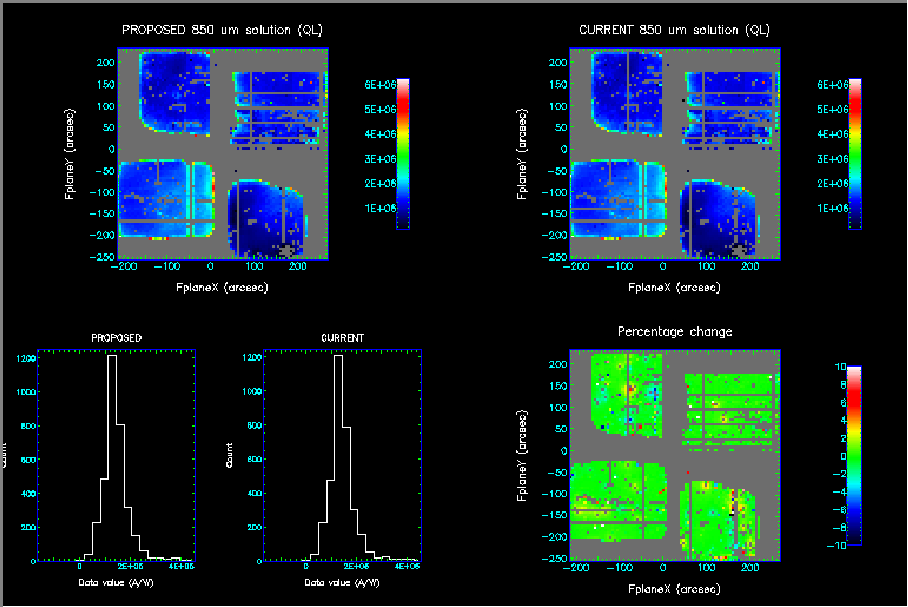
\includegraphics[width=\textwidth]{sun264_flatfield}
\caption{Example display from a FLATFIELD observation or FASTFLAT
  sequence. The top left panel is the responsivity map for this
  observation (containing the proposed new solution), the top right
  panel shows the current responsivity solution (i.e\ currently in
  use) for comparison. The bottom left panels are responsivity
  histograms for this observation and the current solution (PROPOSED
  and CURRENT respectively). The bottom right panel shows the
  percentage change in the responsivities between this observation and
  the current solution in use, scaled between
  $\pm10$\,\%.\label{fig:flatfield}}
\end{figure}

Once complete, the pipeline writes a flag file in
\verb+ORAC_DATA_OUT+ for the current observation containing the name
of each successful flatfield solution. The flag file is a hidden file
with the name \verb+.sYYYYMMDD_MMMMM.ok+ where \verb+YYYYMMDD+ is the
UT date and \verb+MMMMM+ is the zero-padded observation number. This
file is used by the telescope control system (TCS) at the JCMT to
identify the new flatfields to use in subsequent observations.

\subsubsection{Fast-ramps}

The fast-ramp flatfields (FASTFLAT) taken as part of on-sky observing
are included with the science data and processed as part of
map-making, but may be processed separately using the
\task{REDUCE\_FASTFLAT} recipe to assess how much the responsivities
change during an observation. The results are calculated and displayed
as above, but in this case the second fast-ramp flatfield is compared
with the first, and not with the internal flatfield solution.

Fast-ramp flatfields are also processed separately in the QL and
summit pipelines and picked up as necessary for map-making or noise
calculations.

\subsection{NOISE}

Noise observations are a series of measurements recording the
bolometer signal either against a dark shutter or open to the
atmosphere. The telescope is not tracking a source during the
measurement. The recipe calculates the average power spectrum of each
array. The \SMURF\ task \task{calcnoise} is used to calculate the
noise properties for each subarray between 2 and 10\,Hz. The recipe
calibrates the noise data using the appropriate FCF to calculate the
noise equivalent flux density (NEFD). If the measurement is on sky,
the NEFD is also quoted for the zenith, using the current optical
depth and airmass.

A numerical summary of the noise properties, showing the mean, median
and modal noise values, the effective noise equivalent power and
number of bolometers, is written to the screen. These results are also
written to a log file called \verb+log.bolonoise+. The NEFD results
are written to a log file called \verb+log.nefd+.

Focal-plane mosaics of the noise, the percentage change in the noise
since the last measurement and the NEP are displayed in a Kapview
window along with a histogram of the noise values (see
Fig.~\ref{fig:noise}).

The QL and summit pipelines process each file as it is written to
disk. Otherwise all of the data (for a given subarray) are passed to
\task{calcnoise}.

\begin{figure}[t]
\centering
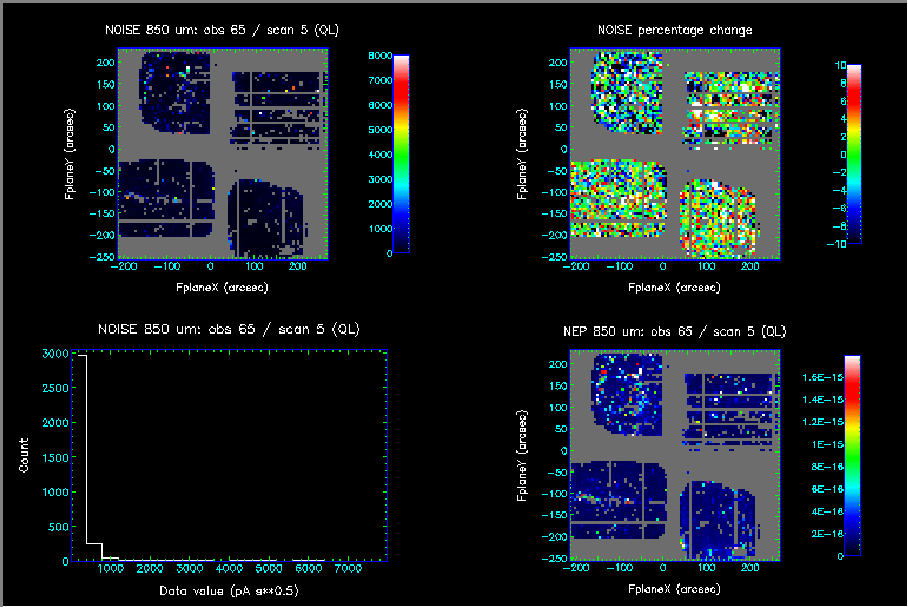
\includegraphics[width=\textwidth]{sun264_noise}
\caption{Example display from a NOISE observation. The top-left panel
  displays the noise for the current data, while the top-right panel
  shows the percentage change since the previous noise
  measurement. The bottom-left panel shows a histogram of noise
  values, while the bottom-right shows the NEP for the current
  data.\label{fig:noise}}
\end{figure}

\subsection{POINTING}

Pointing observations consist of making a map of a point source, and
are processed with the \task{REDUCE\_POINTING} recipe. The recipe
processes the data with the iterative map-maker, crops the image to
75\,arcsec on a side and removes any residual large-scale background
signal with \CUPID\ \task{findback}. If the source is a known
calibrator, the pipeline derives an FCF.

The name of the processed image is written into a flag file (as for
FLATFIELD observations above). The flag file is read by the telescope
POINTING\_FOCUS task which analyzes the named image to calculate the
pointing offsets applied to the telescope pointing model.

The pipeline makes its own estimate of the pointing offsets in two
ways by applying a point-source filter (matched filter) to enhance the
signal-to-noise ratio in the image followed by fitting a 2-D profile
to the source and calculating the centroid position. Both results are
written to a log file called \verb+log.pointing+.

The pipeline displays the image used to derive the pointing offsets in
a \GAIA\ window. The recipe also fits a 2-d profile to the source and
writes the result to a log file called \verb+log.beam+.

The map-maker uses the config file \verb+dimmconfig_pointing.lis+,
except for very short pointing observations (defined as $<15$\,s)
which use \verb+dimmconfig_veryshort_planet.lis+ for planets and
\verb+dimmconfig_bright_compact_veryshort.lis+ for all other sources.

The QL pipeline uses the \task{REDUCE\_POINTING\_QL} recipe, which
contains different logic for dealing with DREAM and STARE data but is
functionally identical to the main \task{REDUCE\_POINTING} recipe for
SCAN data.

\subsection{FOCUS}

Focus observations are processed with the \task{REDUCE\_FOCUS}
recipe. A focus observation consists of a series of maps made of a
point source with the secondary mirror (SMU) at various
positions. Only one axis (either X, Y or Z) is varied at a time.

In the QL pipeline, the maps are made as the data are taken and
collated once the observation has ended. (In practice, due to the fact
that the QL pipeline cannot rely on the \verb+OBSEND+ FITS header, an
observation is considered to have ended once an image exists at each
of the SMU positions: the number of SMU positions is retrieved from
the FITS header.) The non-QL pipeline processes each SMU setting in
turn.

Once all the maps exist, the pipeline creates a cube with the third
axis given by the SMU position. The images are registered to the same
pixel coordinates before adding to the cube so that they align
correctly.

The pipeline writes a flag file (as above) which contains the name of
the data cube. The flag file is read by the telescope POINTING\_FOCUS
task which analyzes the cube to calculate the best SMU position. The
pipeline makes its own estimate of the best-fit SMU position by
fitting a parabola to the peak fluxes derived from 2-D fits (provided
at least three fluxes could be derived) and writes that number to a
log file called \verb+log.focus+.

The images at each focus position are displayed in sequence in a
single Kapview window (see Figure \ref{fig:focus}).

\begin{figure}[t]
\centering
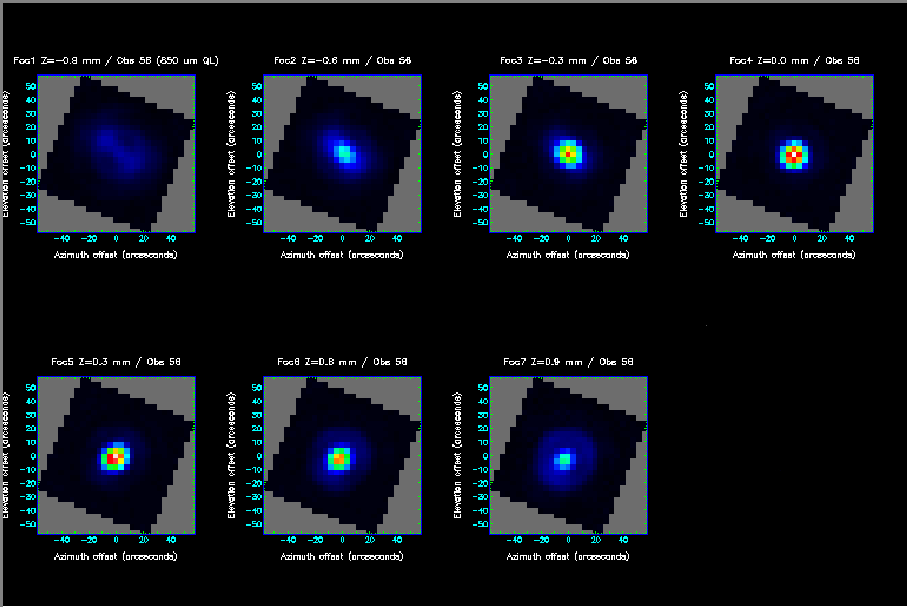
\includegraphics[width=\textwidth]{sun264_focus}
\caption{Example display from a FOCUS observation showing a reduced
  image for each of seven SMU positions. The SMU position (and axis)
  is given in the title for each image. The images are displayed with
  axes of arcsecond offsets.\label{fig:focus}}
\end{figure}

The map-maker uses either the \verb+dimmconfig_veryshort_planet.lis+
for planets and \\ \verb+dimmconfig_bright_compact_veryshort.lis+ for
all other sources.

The same recipe is used for all forms of the pipeline. The output cube
has the suffix \verb+_foc+.

\subsection{SETUP}

A SETUP observation consists of a fast-ramp flatfield (FASTFLAT)
measurement followed by a NOISE, both taken with the shutter
closed. The recipe processes each separately as described for the
respective observation types above. The results of processing each
type of data are displayed in separate Kapview windows. The pipeline
writes a flag file at the end of the observation with the names of the
files containing the names of the flatfield solutions and noise
calculations for the telescope software to read.

\subsection{SKYDIP}

A SKYDIP observation is a series of NOISE-SKY observations at
differing airmass. Currently there is no pipeline recipe to process
these data, other than as a NOISE observation.

\newpage
\section{\xlabel{engineering}Engineering Data\label{se:eng}}

Recipes also exist for processing engineering data, usually taken with
the shutter closed and the telescope stationary. Historically, the
real-time sequencer (RTS) was not involved in such measurements which
prevented the pipeline from processing these data due to missing FITS
headers and other essential metadata.

In September 2010 is was decided that the pipeline be used to process
and analyze data taken in engineering mode, and a simulated RTS is
used to generate metadata. Support for engineering data is currently
quite rudimentary with only a single recipe available.

Note that in order to process data taken in engineering mode, the
\verb+-eng+ option must be given to the \oracdr\ initialization
script.

\subsection{NEP}

Measurements of the noise-equivalent power (NEP) are processed with
the \task{ENG\_NEP} recipe. The `observation' consists of a series of
NOISE measurements at different pixel heater and detector bias
values. The recipe is designed to run offline, after the observation
has finished.

The NEP is calculated for each subarray at each setting. These
per-bolometer NEP images are combined to form a 4-d hypercube with
axes bolometer row, bolometer column, heater setting and bias setting
for each subarray. These hypercubes are named
\verb+sXXYYYYMMDD_MMMMM_nep.sdf+ where \verb+sXX+ is the subarray
label (e.g.\ \verb+s8a+).

From these data, the effective and RMS NEP is calculated at each
heater and bias setting, stored as a 2-d image with the heater and
bias values as the X- and Y axes. These images have suffices of
\verb+_effnep+ and \verb+_rmsnep+ respectively.

A number of log files are also written. The first is called
\verb+log.bolonoise+ which contains the noise properties for each
heater and bias setting and all subarrays. Log files for the `mapping
speed' parameter for each subarray are written separately with the
name \verb+log.mapspeed_SXX+ where \verb+SXX+ is the subarray
(e.g.\ s4a). The mapping speed is given by $N_{\rm bol} / {\rm
  NEP}_{\rm RMS}^2$ and is calculated for the best $N_{\rm bol}$
bolometers between 300 and 1000 in steps of 100 bolometers.

The recipe does not display any data.

\newpage

\section{\xlabel{ap_list}Alphabetical list of SCUBA-2 recipes\label{ap:list}}

\begin{description}
\menuitem{ARRAY\_TESTS}{
  Co-add and display DREAM/STARE images}
\menuitem{ASSESS\_DATA\_NOISE}{
  Calculate noise properties of SCUBA-2 data}
\menuitem{BENCHMARK}{
  Benchmarking recipe}
\menuitem{ENG\_NEP}{
  Process NEP measurements made in engineering mode}
\menuitem{ENG\_NEP\_QL}{
  Process NEP measurements made in engineering mode using the QL pipeline}
\menuitem{FAINT\_POINT\_SOURCES}{
  Process SCAN data from faint compact sources}
\menuitem{FAINT\_POINT\_SOURCES\_JACKKNIFE}{
  Process blank field data with a jack-knife-based method}
\menuitem{REDUCE\_CLS}{
  Process data taken as part of the CLS JCMT legacy survey}
\menuitem{REDUCE\_DARK}{
  Process dark frames}
\menuitem{REDUCE\_DREAMSTARE}{
  Process DREAM/STARE images}
\menuitem{REDUCE\_DREAMSTARE\_QL}{
  QL processing DREAM/STARE images}
\menuitem{REDUCE\_FASTFLAT}{
  Process fast-ramp flatfield data}
\menuitem{REDUCE\_FLATFIELD}{
  Process flatfield measurements}
\menuitem{REDUCE\_FOCUS}{
  Recipe for deriving focus information}
\menuitem{REDUCE\_FOCUS\_QL}{
  process focus observations in the quick-look pipeline}
\menuitem{REDUCE\_FOCUS\_SUMMIT}{
  derive focus information in the summit pipeline}
\menuitem{REDUCE\_FTS\_FOCUS}{
  Recipe for processing FTS-2 focus observations}
\menuitem{REDUCE\_FTS\_IMAGE\_FOCUS}{
  Recipe for processing FTS-2 image focus observations}
\menuitem{REDUCE\_FTS\_IMAGE\_POINTING}{
  Recipe for processing FTS-2 image pointing observations}
\menuitem{REDUCE\_FTS\_POINTING}{
  Recipe for processing FTS-2 pointing observations}
\menuitem{REDUCE\_FTS\_SCAN}{
  Recipe for processing FTS-2 SCAN data}
\menuitem{REDUCE\_FTS\_SCAN\_QL}{
  Recipe for processing FTS-2 SCAN data in the QL pipeline}
\menuitem{REDUCE\_FTS\_SCAN\_SUMMIT}{
  Recipe for processing FTS-2 SCAN data in the SUMMIT pipeline}
\menuitem{REDUCE\_FTS\_ZPD}{
  Recipe for processing FTS-2 SCAN data}
\menuitem{REDUCE\_FTS\_ZPD\_QL}{
  Recipe for processing FTS-2 SCAN data in the QL pipeline}
\menuitem{REDUCE\_FTS\_ZPD\_SUMMIT}{
  Recipe for processing FTS-2 SCAN data in the SUMMIT pipeline}
\menuitem{REDUCE\_JPS}{
  Process data taken as part of the JPS JCMT legacy survey}
\menuitem{REDUCE\_NOISE}{
  Process NOISE observations}
\menuitem{REDUCE\_NOISE\_PHOTON}{
  Determine photon noise contribution to total noise}
\menuitem{REDUCE\_NOISE\_QL}{
  QL processing NOISE observations}
\menuitem{REDUCE\_NOISE\_SUMMIT}{
  SUMMIT processing NOISE observations}
\menuitem{REDUCE\_POINTING}{
  Process POINTING observations}
\menuitem{REDUCE\_POINTING\_CADC}{
  Process pointing data at CADC}
\menuitem{REDUCE\_POINTING\_QL}{
  QL processing of pointing observations}
\menuitem{REDUCE\_POINTING\_SUMMIT}{
  Summit processing of pointing observations}
\menuitem{REDUCE\_POL\_STARE}{
  Recipe for processing POL-2 stare data}
\menuitem{REDUCE\_POL\_STARE\_QL}{
  Recipe for processing POL-2 stare data in the QL pipeline}
\menuitem{REDUCE\_POL\_STARE\_SUMMIT}{
  Recipe for processing POL-2 stare data in the SUMMIT pipeline}
\menuitem{REDUCE\_SASSY}{
  Process data for the SASSy JCMT legacy survey}
\menuitem{REDUCE\_SASSY\_QL}{
  Process data for the SASSy JCMT legacy survey in the QL pipeline}
\menuitem{REDUCE\_SASSY\_SUMMIT}{
  Process data for the SASSy JCMT legacy survey in the SUMMIT pipeline}
\menuitem{REDUCE\_SCAN}{
  Process SCAN-mode data}
\menuitem{REDUCE\_SCAN\_CHECKRMS}{
  Process scan data and collect noise/NEFD statistics}
\menuitem{REDUCE\_SCAN\_EXTENDED\_SOURCES}{
  Process SCAN data from extended sources}
\menuitem{REDUCE\_SCAN\_EXTENDED\_SOURCES\_QL}{
  Process SCAN data from extended sources in the QL pipeline}
\menuitem{REDUCE\_SCAN\_EXTENDED\_SOURCES\_SUMMIT}{
  Process SCAN data from extended sources in the SUMMIT pipeline}
\menuitem{REDUCE\_SCAN\_FAINT\_POINT\_SOURCES}{
  Process SCAN data from faint compact sources}
\menuitem{REDUCE\_SCAN\_FAINT\_POINT\_SOURCES\_JACKKNIFE}{
  Process blank field data with a jack-knife-based method}
\menuitem{REDUCE\_SCAN\_FAINT\_POINT\_SOURCES\_QL}{
  Process SCAN data from faint compact sources in the QL pipeline}
\menuitem{REDUCE\_SCAN\_FAINT\_POINT\_SOURCES\_SUMMIT}{
  Process SCAN data from faint compact sources in the SUMMIT pipeline}
\menuitem{REDUCE\_SCAN\_FAKEMAP}{
  Process SCAN data with existing map data added}
\menuitem{REDUCE\_SCAN\_JSA\_PUBLIC}{
  Form observation tiles for the public co-add}
\menuitem{REDUCE\_SCAN\_QL}{
  QL process SCAN data}
\menuitem{REDUCE\_SCAN\_SUMMIT}{
  Summit recipe for processing SCAN data}
\menuitem{REDUCE\_SETUP}{
  Process data from a setup observation}
\menuitem{REDUCE\_SETUP\_QL}{
  Process data from a setup observation in the QL pipeline}
\menuitem{REDUCE\_SETUP\_SUMMIT}{
  Process data from a setup observation in the SUMMIT pipeline}
\menuitem{REDUCE\_SKYDIP}{
  Process SKYDIP observations}
\menuitem{REDUCE\_SKYDIP\_QL}{
  Process SKYDIP observations in the QL pipeline}
\menuitem{REDUCE\_SKYDIP\_SUMMIT}{
  Process SKYDIP observations in the SUMMIT pipeline}
\menuitem{REDUCE\_SONS}{
  Process data taken as part of the SONS JCMT legacy survey}
\end{description}


\newpage
\begin{small}
\section{\xlabel{ap_classified}Classified list of SCUBA-2 recipes\label{ap:classified}}

SCUBA-2 recipes may be classified in terms of their observing mode as
follows.

{\large
\begin{center}
\textbf{Science data: SCAN mode}
\end{center}
}

\begin{description}
\classitem{FAINT\_POINT\_SOURCES}
Process SCAN data from faint compact sources
\classitem{FAINT\_POINT\_SOURCES\_JACKKNIFE}
Process blank field data with a jack-knife-based method
\classitem{REDUCE\_CLS}
Process data taken as part of the CLS JCMT legacy survey
\classitem{REDUCE\_JPS}
Process data taken as part of the JPS JCMT legacy survey
\classitem{REDUCE\_SASSY}
Process data for the SASSy JCMT legacy survey
\classitem{REDUCE\_SASSY\_QL}
Process data for the SASSy JCMT legacy survey in the QL pipeline
\classitem{REDUCE\_SASSY\_SUMMIT}
Process data for the SASSy JCMT legacy survey in the SUMMIT pipeline
\classitem{REDUCE\_SCAN}
Process SCAN-mode data
\classitem{REDUCE\_SCAN\_CHECKRMS}
Process scan data and collect noise/NEFD statistics
\classitem{REDUCE\_SCAN\_EXTENDED\_SOURCES}
Process SCAN data from extended sources
\classitem{REDUCE\_SCAN\_EXTENDED\_SOURCES\_QL}
Process SCAN data from extended sources in the QL pipeline
\classitem{REDUCE\_SCAN\_EXTENDED\_SOURCES\_SUMMIT}
Process SCAN data from extended sources in the SUMMIT pipeline
\classitem{REDUCE\_SCAN\_FAINT\_POINT\_SOURCES}
Process SCAN data from faint compact sources
\classitem{REDUCE\_SCAN\_FAINT\_POINT\_SOURCES\_JACKKNIFE}
Process blank field data with a jack-knife-based method
\classitem{REDUCE\_SCAN\_FAINT\_POINT\_SOURCES\_QL}
Process SCAN data from faint compact sources in the QL pipeline
\classitem{REDUCE\_SCAN\_FAINT\_POINT\_SOURCES\_SUMMIT}
Process SCAN data from faint compact sources in the SUMMIT pipeline
\classitem{REDUCE\_SCAN\_FAKEMAP}
Process SCAN data with existing map data added
\classitem{REDUCE\_SCAN\_JSA\_PUBLIC}
Form observation tiles for the public co-add
\classitem{REDUCE\_SCAN\_QL}
QL process SCAN data
\classitem{REDUCE\_SCAN\_SUMMIT}
Summit recipe for processing SCAN data
\classitem{REDUCE\_SONS}
Process data taken as part of the SONS JCMT legacy survey
\end{description}

{\large
\begin{center}
\textbf{Science data: DREAM/STARE mode}
\end{center}
}
\begin{description}
\classitem{REDUCE\_DREAMSTARE}
Process DREAM/STARE images
\classitem{REDUCE\_DREAMSTARE\_QL}
QL processing DREAM/STARE images
\end{description}

{\large
\begin{center}
\textbf{Science data: FTS-2}
\end{center}
}
\begin{description}
\classitem{REDUCE\_FTS\_SCAN}
Recipe for processing FTS-2 SCAN data
\classitem{REDUCE\_FTS\_SCAN\_QL}
Recipe for processing FTS-2 SCAN data in the QL pipeline
\classitem{REDUCE\_FTS\_SCAN\_SUMMIT}
Recipe for processing FTS-2 SCAN data in the SUMMIT pipeline
\classitem{REDUCE\_FTS\_ZPD}
Recipe for processing FTS-2 SCAN data
\classitem{REDUCE\_FTS\_ZPD\_QL}
Recipe for processing FTS-2 SCAN data in the QL pipeline
\classitem{REDUCE\_FTS\_ZPD\_SUMMIT}
Recipe for processing FTS-2 SCAN data in the SUMMIT pipeline
\end{description}

{\large
\begin{center}
\textbf{Science data: POL-2}
\end{center}
}
\begin{description}
\classitem{REDUCE\_POL\_STARE}
Recipe for processing POL-2 stare data
\classitem{REDUCE\_POL\_STARE\_QL}
Recipe for processing POL-2 stare data in the QL pipeline
\classitem{REDUCE\_POL\_STARE\_SUMMIT}
Recipe for processing POL-2 stare data in the SUMMIT pipeline
\end{description}

{\large
\begin{center}
\textbf{Pointing observations}
\end{center}
}
\begin{description}
\classitem{REDUCE\_FTS\_IMAGE\_POINTING}
Recipe for processing FTS-2 image pointing observations
\classitem{REDUCE\_FTS\_POINTING}
Recipe for processing FTS-2 pointing observations
\classitem{REDUCE\_POINTING}
Process POINTING observations
\classitem{REDUCE\_POINTING\_QL}
QL processing of pointing observations
\classitem{REDUCE\_POINTING\_SUMMIT}
Summit processing of pointing observations
\end{description}

{\large
\begin{center}
\textbf{Focus observations}
\end{center}
}
\begin{description}
\classitem{REDUCE\_FTS\_FOCUS}
Recipe for processing FTS-2 focus observations
\classitem{REDUCE\_FTS\_IMAGE\_FOCUS}
Recipe for processing FTS-2 image focus observations
\classitem{REDUCE\_FOCUS}
Recipe for deriving focus information
\classitem{REDUCE\_FOCUS\_QL}
process focus observations in the quick-look pipeline
\classitem{REDUCE\_FOCUS\_SUMMIT}
derive focus information in the summit pipeline
\end{description}

{\large
\begin{center}
\textbf{Noise observations}
\end{center}
}
\begin{description}
\classitem{ASSESS\_DATA\_NOISE}
Calculate noise properties of SCUBA-2 data
\classitem{ENG\_NEP}
Process NEP measurements made in engineering mode
\classitem{ENG\_NEP\_QL}
Process NEP measurements made in engineering mode using the QL pipeline
\classitem{REDUCE\_NOISE}
Process NOISE observations
\classitem{REDUCE\_NOISE\_PHOTON}
Determine photon noise contribution to total noise
\classitem{REDUCE\_NOISE\_QL}
QL processing NOISE observations
\classitem{REDUCE\_NOISE\_SUMMIT}
SUMMIT processing NOISE observations
\classitem{REDUCE\_SKYDIP}
Process SKYDIP observations
\classitem{REDUCE\_SKYDIP\_QL}
Process SKYDIP observations in the QL pipeline
\classitem{REDUCE\_SKYDIP\_SUMMIT}
Process SKYDIP observations in the SUMMIT pipeline
\end{description}

{\large
\begin{center}
\textbf{Flatfield observations}
\end{center}
}
\begin{description}
\classitem{REDUCE\_FASTFLAT}
Process fast-ramp flatfield data
\classitem{REDUCE\_FLATFIELD}
Process flatfield measurements
\end{description}

{\large
\begin{center}
\textbf{Setup observations}
\end{center}
}
\begin{description}
\classitem{REDUCE\_SETUP}
Process data from a setup observation
\classitem{REDUCE\_SETUP\_QL}
Process data from a setup observation in the QL pipeline
\classitem{REDUCE\_SETUP\_SUMMIT}
Process data from a setup observation in the SUMMIT pipeline
\end{description}

{\large
\begin{center}
\textbf{QL-pipeline recipes}
\end{center}
}
\begin{description}
\classitem{ENG\_NEP\_QL}
Process NEP measurements made in engineering mode using the QL pipeline
\classitem{REDUCE\_DREAMSTARE\_QL}
QL processing DREAM/STARE images
\classitem{REDUCE\_FOCUS\_QL}
process focus observations in the quick-look pipeline
\classitem{REDUCE\_FTS\_SCAN\_QL}
Recipe for processing FTS-2 SCAN data in the QL pipeline
\classitem{REDUCE\_FTS\_ZPD\_QL}
Recipe for processing FTS-2 SCAN data in the QL pipeline
\classitem{REDUCE\_NOISE\_QL}
QL processing NOISE observations
\classitem{REDUCE\_POINTING\_QL}
QL processing of pointing observations
\classitem{REDUCE\_POL\_STARE\_QL}
Recipe for processing POL-2 stare data in the QL pipeline
\classitem{REDUCE\_SASSY\_QL}
Process data for the SASSy JCMT legacy survey in the QL pipeline
\classitem{REDUCE\_SCAN\_EXTENDED\_SOURCES\_QL}
Process SCAN data from extended sources in the QL pipeline
\classitem{REDUCE\_SCAN\_FAINT\_POINT\_SOURCES\_QL}
Process SCAN data from faint compact sources in the QL pipeline
\classitem{REDUCE\_SCAN\_QL}
QL process SCAN data
\classitem{REDUCE\_SETUP\_QL}
Process data from a setup observation in the QL pipeline
\classitem{REDUCE\_SKYDIP\_QL}
Process SKYDIP observations in the QL pipeline
\end{description}

{\large
\begin{center}
\textbf{Summit-pipeline recipes}
\end{center}
}
\begin{description}
\classitem{REDUCE\_FOCUS\_SUMMIT}
Derive focus information in the summit pipeline
\classitem{REDUCE\_FTS\_SCAN\_SUMMIT}
Recipe for processing FTS-2 SCAN data in the SUMMIT pipeline
\classitem{REDUCE\_FTS\_ZPD\_SUMMIT}
Recipe for processing FTS-2 SCAN data in the SUMMIT pipeline
\classitem{REDUCE\_NOISE\_SUMMIT}
SUMMIT processing NOISE observations
\classitem{REDUCE\_POINTING\_SUMMIT}
Summit processing of pointing observations
\classitem{REDUCE\_POL\_STARE\_SUMMIT}
Recipe for processing POL-2 stare data in the SUMMIT pipeline
\classitem{REDUCE\_SASSY\_SUMMIT}
Process data for the SASSy JCMT legacy survey in the SUMMIT pipeline
\classitem{REDUCE\_SCAN\_EXTENDED\_SOURCES\_SUMMIT}
Process SCAN data from extended sources in the SUMMIT pipeline
\classitem{REDUCE\_SCAN\_FAINT\_POINT\_SOURCES\_SUMMIT}
Process SCAN data from faint compact sources in the SUMMIT pipeline
\classitem{REDUCE\_SCAN\_SUMMIT}
Summit recipe for processing SCAN data
\classitem{REDUCE\_SETUP\_SUMMIT}
Process data from a setup observation in the summit pipeline
\classitem{REDUCE\_SKYDIP\_SUMMIT}
Process SKYDIP observations with the summit pipeline
\end{description}

{\large
\begin{center}
\textbf{Miscellaneous}
\end{center}
}
\begin{description}
\classitem{ARRAY\_TESTS}
Co-add and display DREAM/STARE images
\classitem{BENCHMARK}
Benchmarking recipe
\classitem{REDUCE\_DARK}
Process dark frames
\end{description}


\end{small}


\section{Main Science recipes}
\input{mainrecipes}

\section{FTS-2 recipes}
\input{fts}

\section{POL-2 recipes}
\input{pol}

\section{Summit Recipes}
\input{summit}

\section{Quick Look Recipes}
\input{quicklook}

\section{Recipes for Non Science Observations}
\input{nonscience}

\section{Obsolete Recipes}
\input{obsolete}

\end{document}

